\title{Probabilistic PCA}

\subsection{Probabilistic PCA}

Probabilistic principal components analysis (PCA) is a
dimensionality reduction technique that
analyzes data via a lower dimensional latent space
\citep{tipping1999probabilistic}. It is often
used when there are missing values in the data or for multidimensional
scaling.

We demonstrate with an example in Edward.
An interactive version with Jupyter notebook is available
\href{http://nbviewer.jupyter.org/github/blei-lab/edward/blob/master/notebooks/probabilistic_pca.ipynb}{here}.

\subsubsection{Data}

We use simulated data. We'll talk about the individual variables and
what they stand for in the next section. For this example, each data
point is 2-dimensional, $\mathbf{x}_n\in\mathbb{R}^2$.

\begin{lstlisting}[language=Python]
def build_toy_dataset(N, D, K, sigma=1):
  x_train = np.zeros((D, N))
  w = np.random.normal(0.0, 2.0, size=(D, K))
  z = np.random.normal(0.0, 1.0, size=(K, N))
  mean = np.dot(w, z)
  for d in range(D):
    for n in range(N):
      x_train[d, n] = np.random.normal(mean[d, n], sigma)

  print("True principal axes:")
  print(w)
  return x_train

N = 5000  # number of data points
D = 2  # data dimensionality
K = 1  # latent dimensionality

x_train = build_toy_dataset(N, D, K)
\end{lstlisting}

\begin{lstlisting}
## True principal axes:
## [[ 0.25947927]
##  [ 1.80472372]]
\end{lstlisting}

We visualize the data set.

\begin{lstlisting}[language=Python]
plt.scatter(x_train[0, :], x_train[1, :], color='blue', alpha=0.1)
plt.axis([-10, 10, -10, 10])
plt.title("Simulated data set")
plt.show()
\end{lstlisting}

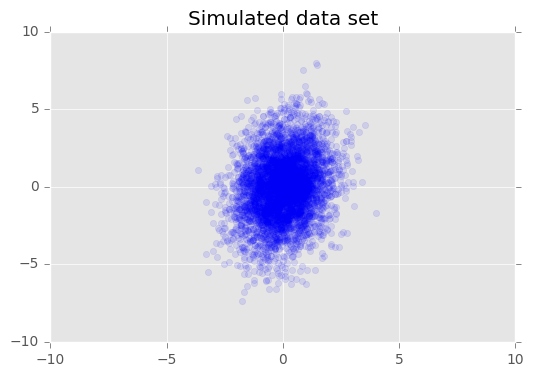
\includegraphics[width=450px]{/images/probabilistic-pca-fig0.png}

\subsubsection{Model}

Consider a data set $\mathbf{X} = \{\mathbf{x}_n\}$ of $N$ data
points, where each data point is $D$-dimensional, $\mathbf{x}_n \in
\mathbb{R}^D$. We aim to represent each $\mathbf{x}_n$ under a latent
variable $\mathbf{z}_n \in \mathbb{R}^K$ with lower dimension, $K <
D$. The set of principal axes $\mathbf{W}$ relates the latent variables to
the data.

Specifically, we assume that each latent variable is normally distributed,
\begin{equation*}
\mathbf{z}_n \sim N(\mathbf{0}, \mathbf{I}).
\end{equation*}
The corresponding data point is generated via a projection,
\begin{equation*}
\mathbf{x}_n \mid \mathbf{z}_n
\sim N(\mathbf{W}\mathbf{z}_n, \sigma^2\mathbf{I}),
\end{equation*}
where the matrix $\mathbf{W}\in\mathbb{R}^{D\times K}$ are known as
the principal axes. In probabilistic PCA, we are typically interested in
estimating the principal axes $\mathbf{W}$ and the noise term
$\sigma^2$.

Probabilistic PCA generalizes classical PCA. Marginalizing out the the
latent variable, the distribution of each data point is
\begin{equation*}
\mathbf{x}_n \sim N(\mathbf{0}, \mathbf{W}\mathbf{W}^Y + \sigma^2\mathbf{I}).
\end{equation*}
Classical PCA is the specific case of probabilistic PCA when the
covariance of the noise becomes infinitesimally small, $\sigma^2 \to
0$.

We set up our model below. In our analysis, we fix $\sigma=2.0$, and
instead of point estimating $\mathbf{W}$ as a model parameter, we
place a prior over it in order to infer a distribution over principal
axes.

\begin{lstlisting}[language=Python]
from edward.models import Normal

w = Normal(loc=tf.zeros([D, K]), scale=2.0 * tf.ones([D, K]))
z = Normal(loc=tf.zeros([N, K]), scale=tf.ones([N, K]))
x = Normal(loc=tf.matmul(w, z, transpose_b=True), scale=tf.ones([D, N]))

\end{lstlisting}

\subsubsection{Inference}

The posterior distribution over the principal axes $\mathbf{W}$ cannot
be analytically determined. Below, we set up our inference variables
and then run a chosen algorithm to infer $\mathbf{W}$. Below we use
variational inference to minimize the $\text{KL}(q\|p)$ divergence
measure.

\begin{lstlisting}[language=Python]
qw = Normal(loc=tf.Variable(tf.random_normal([D, K])),
            scale=tf.nn.softplus(tf.Variable(tf.random_normal([D, K]))))
qz = Normal(loc=tf.Variable(tf.random_normal([N, K])),
            scale=tf.nn.softplus(tf.Variable(tf.random_normal([N, K]))))

inference = ed.KLqp({w: qw, z: qz}, data={x: x_train})
inference.run(n_iter=500, n_print=100, n_samples=10)
\end{lstlisting}

\subsubsection{Criticism}

To check our inferences, we first inspect the model's learned
principal axes.

\begin{lstlisting}[language=Python]
sess = ed.get_session()
print("Inferred principal axes:")
print(sess.run(qw.mean()))
\end{lstlisting}

\begin{lstlisting}
## Inferred principal axes:
## [[-0.24093632]
##  [-1.76468039]]
\end{lstlisting}

The model has recovered the true principal axes up to finite data and
also up to identifiability (there's a symmetry in the
parameterization).

Another way to criticize the model is to visualize the observed data
against data generated from our fitted model.

\begin{lstlisting}[language=Python]
x_post = ed.copy(x, {w: qw, z: qz})
x_gen = sess.run(x_post)

plt.scatter(x_gen[0, :], x_gen[1, :], color='red', alpha=0.1)
plt.axis([-10, 10, -10, 10])
plt.title("Data generated from model")
plt.show()
\end{lstlisting}

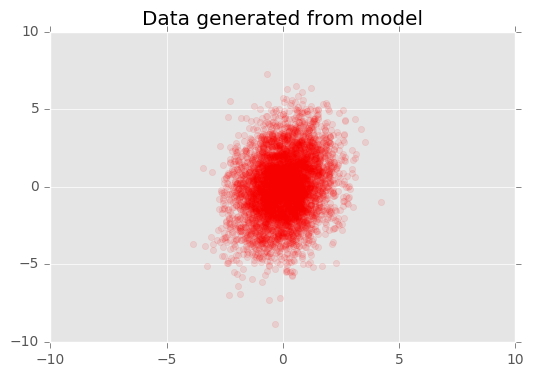
\includegraphics[width=450px]{/images/probabilistic-pca-fig1.png}

The generated data looks close to the true data.

\subsubsection{Acknowledgments}

We thank Mayank Agrawal for writing the initial version of this
tutorial.

\subsubsection{References}\label{references}
